\section{Results}
\label{sec:results}

To thoroughly assess the performance of the controllers and estimators \& filters, several reference signals were designed to evaluate different aspects of system dynamics, including transient response, steady-state behavior, adaptability, and robustness.

In the following sections, we propose:

\begin{itemize}
    \item \textbf{Controllers comparison}: a comparison between PIDs, LQs and MPC controllers as designed in Section \ref{sec:controllers_design}. Results are obtained using Kalman filters to estimate and/or filter the system's state.
    \item \textbf{Filters comparison}: a comparison between the filters designed in Section \ref{sec:filters_estimators_design}. Results are obtained using an LQR tracking controller to evaluate the observer's ability to track the system's state during continuous oscillatory motion.
\end{itemize}

\subsection{Controllers comparison}
\label{subsec:controllers_comparison}

In the following sections, controllers designed in Section \ref{sec:controllers_design} are compared using different reference inputs signals.

As stated in the introduction, all the results here presented are obtained using a Kalman filter to estimate and/or filter the system's state.

\subsubsection{Multi-steps reference}
\label{subsubsec:multisteps_reference}

A sequence of equally spaced step inputs is designed to assess the controller's response to abrupt set-point changes and its steady-state performance across various set-points.

Two versions of the multi-steps reference signals are explored:

\begin{itemize}
    \item \textbf{Up \& down}: signal designed to evaluate the controller's performance by moving the sphere in both directions relative to the linearization point, using steps of amplitude $2 [mm]$.
          This test assesses the controller's ability to maintain stability and accuracy during repeated set-point changes, as well as its robustness in handling deviations in both directions.
    \item \textbf{Stairs}: signal with steps always in the same direction, ranging from $8 [mm]$ to $12 [mm]$ with a resolution of $1 [mm]$.
          This test is particularly useful for analyzing the controller's response to minor perturbations and its capacity for gradual positional adjustments.
\end{itemize}

The following figures show the comparison of the controllers using the multi-steps reference signals.

\begin{figure}[H]
    \centering
    \includegraphics[width=1\linewidth]{./img/MATLAB/results/multisteps_stairs_star_KF.pdf}
    \caption{Comparison of controllers with multistep stairs reference using KF}
\end{figure}

\begin{figure}[H]
    \centering
    \includegraphics[width=1\linewidth]{./img/MATLAB/results/multisteps_updown_star_KF.pdf}
    \caption{Comparison of controllers with multistep up \& down reference using KF}
\end{figure}

\begin{figure}[H]
    \centering
    \includegraphics[width=0.32\linewidth]{./img/MATLAB/results/multisteps_up_PIDstar_KF.pdf}
    \hfill
    \includegraphics[width=0.32\linewidth]{./img/MATLAB/results/multisteps_up_LQstar_KF.pdf}
    \hfill
    \includegraphics[width=0.32\linewidth]{./img/MATLAB/results/multisteps_up_MPCstar_KF.pdf}
    \caption{PIDs, LQs, MPC with multistep up reference using KF}
\end{figure}

\begin{figure}[H]
    \centering
    \includegraphics[width=0.32\linewidth]{./img/MATLAB/results/multisteps_down_PIDstar_KF.pdf}
    \hfill
    \includegraphics[width=0.32\linewidth]{./img/MATLAB/results/multisteps_down_LQstar_KF.pdf}
    \hfill
    \includegraphics[width=0.32\linewidth]{./img/MATLAB/results/multisteps_down_MPCstar_KF.pdf}
    \caption{PIDs, LQs, MPC with multistep up \& down (down) reference using KF}
\end{figure}

\paragraph{PID anti-windup}

The PID anti-windup controller exhibits the response that deviates the most from the reference data compared to the other developed controllers.

The trajectory presents an overshoot before the sphere approaches the correct value.
This behavior clearly delays the achievement of the reference position.
In fact the sphere reaches the reference position just in time before it is changed.

The control exhibits numerous oscillations and peaks, particularly during transitions.

The slowness in approaching the target position makes the PID anti-windup unsuitable for rapid reference changes.

\paragraph{PID gain scheduling}

According to the theory, the performance of the PID, is significantly enhanced by the development of PID gain scheduling.

Using multiple linearization, it enables a much more accurate trajectory of the sphere, free from overshoots and considerably faster.

Additionally, the control behavior in the case of PID gain scheduling is cleaner respect to the anti-windup case, but not respect to the other controllers.

The effectiveness of PID gain scheduling is limited by the linearity of the model: in the presence of non-linearities or complex dynamics, it cannot compete with advanced techniques such as LQR or LQI.

\paragraph{LQR tracking}

The LQR tracking controller exhibits reduced error during the transient phase, with small oscillations as the set points are reached.
In steady state, the error is small, but the accuracy can be enhanced by the use of LQI controller.
A small overshoot peak is observed prior to stabilization.

Dynamically, the response is very fast, demonstrating that LQR tracking is the quickest controller among those implemented.

The control behavior is highly smooth and significantly outperforms both the PID anti-windup and the PID gain scheduling.
The control signal presents some peaks during the steps, but they remain well-contained.

The small oscillations observed are due to the lack of an integral component, which does not allow to completely cancel constant errors.

\paragraph{LQI}

The LQI controller, leveraging its integral term, compensates the accumulated error over time.
In steady state, the sphere approaches the reference trajectory with smaller discrepancy compared to the LQR tracking case.

Dynamically, the transitions are less aggressive, and the overshoot is reduced, at the cost of a slightly increased stabilization time.

The control exhibits small fluctuations and avoids the peaks observed in the tracking case.
The LQI control establishes itself as the cleanest control signal, as demonstrated in all the figures above.

The slower stabilization is a consequence of the more controlled and less aggressive dynamics compared to LQR.

Compared to the LQR, the LQI is particularly suitable for applications where stability and accuracy are more important than response speed.

\paragraph{MPC}

The MPC exhibits a more oscillatory behavior compared to LQR or LQI, with pronounced oscillations during set point transitions.
These oscillations are particularly noticeable at reference step changes.

In steady-state conditions, the MPC sufficiently reduces the error, stabilizing more slowly than LQI and PID gain scheduling, but faster than the PID anti-windup.

The MPC is more aggressive in attempting to reach the set point.

The control graph shows oscillations and peaks during position changes, which remain contained.

The MPC control is less smooth than LQI and LQR tracking but is better respect both the PID controllers.
MPC is best suited for complex, multivariable scenarios, but in cases with rapid transitions it may be less smooth than LQR and LQI.



\subsubsection{Sinusoidal (discrete) reference}
\label{subsubsec:sinusoidal_discrete_reference}

As a second reference signal for the comparison of the controllers, we propose the sinusoidal (discrete) reference.

Here the input signal is a sinusoidal shape, but represented as a sequence of discrete steps.
The period on the sinusoidal is 2 seconds, and the amplitude is $2 [mm]$ centered around $10 [mm]$.

The following figures show the comparison of the controllers using the sinusoidal reference signals.

\begin{figure}[H]
    \centering
    \includegraphics[width=1\linewidth]{./img/MATLAB/results/sinusoidal_fast_star_KF.pdf}
    \caption{Comparison of controllers with sinusoidal fast reference using KF}
\end{figure}

\begin{figure}[H]
    \centering
    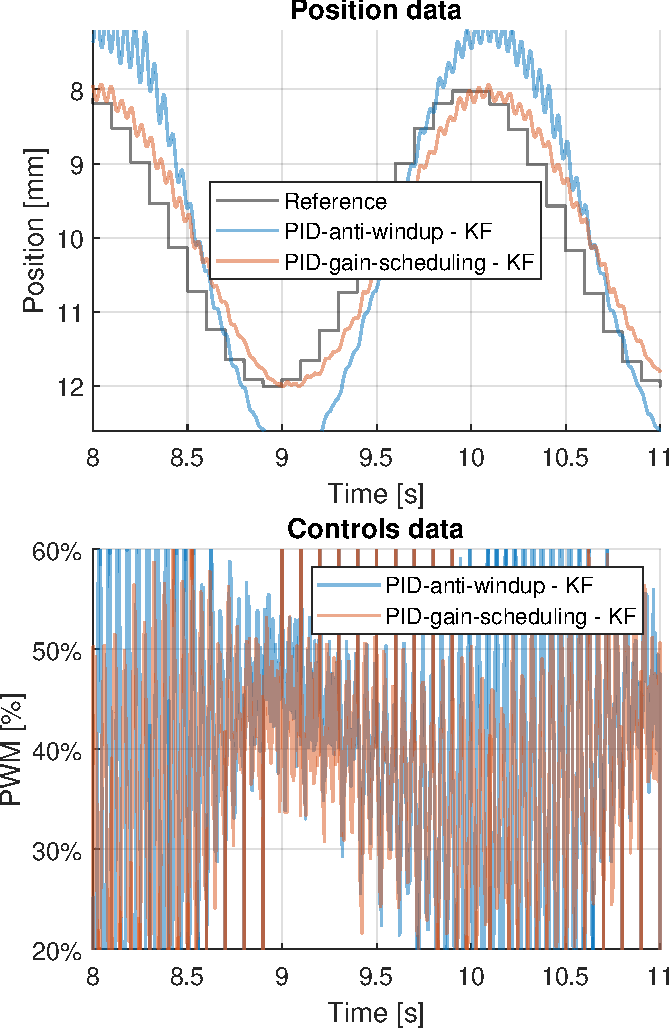
\includegraphics[width=0.32\linewidth]{./img/MATLAB/results/sinusoidal_fast_PIDstar_KF.pdf}
    \hfill
    \includegraphics[width=0.32\linewidth]{./img/MATLAB/results/sinusoidal_fast_LQstar_KF.pdf}
    \hfill
    \includegraphics[width=0.32\linewidth]{./img/MATLAB/results/sinusoidal_fast_MPCstar_KF.pdf}
    \caption{PIDs, LQs, MPC with sinusoidal fast reference using KF}
\end{figure}

\paragraph{PID anti-windup}

As with the multistep reference, in the case of the fast sine reference, the PID anti-windup controller proves to be the least effective.
The nature of the PID and the inability to anticipate dynamics make it difficult to manage a rapidly varying trajectory such as a stepped sine.

It deviates from the desired trajectory much more significantly compared to the other controllers developed and exhibits greater oscillations, particularly when the sphere is closer to the upper coil.

The control performance is also the worst when compared to the other controllers, with large oscillations at the extreme points of the sine wave.

\paragraph{PID gain scheduling}

The PID gain scheduling significantly reduces oscillations of the trajectory, as observed in the multistep reference, demonstrating a much better performance than the anti-windup case.
However, it still shows oscillations, particularly when the sphere reaches a distance of 8 mm from the upper coil.

The control remains really inadequate with large oscillations, in particular at the extreme points of the sinusoidal.

\paragraph{LQR tracking}

The LQR tracking is highly accurate, with the trajectory closely following the reference and exhibiting small oscillations.
The control is much improved, without saturation and very low oscillations.


\paragraph{LQI}

The LQI, thanks to its integral term, is able to follow the reference even more precisely than the LQR tracking.
It once again proves to be the best controller for achieving an accurate and fast response with very clean control.

The control signal is smooth, without peaks or large oscillations.
The fast sine reference demonstrates the great performance of this controller.
The LQI is able to manage not only the dynamic trajectory, but also to maintain a practically zero error at steady state, proving to be the cleanest and most stable.

\paragraph{MPC}

Despite some trajectory delay due to prediction calculations, the MPC is able to follow the reference, proving to be a sufficient controller even for a fast dynamic system like this one.

The control exhibits several peaks, but they are always well contained.
As it was written for the multistep case, MPC is best suited for complex, multivariable scenarios, but in this case the performance is inferior respect to LQR tracking and LQI.



\subsubsection{Conclusions}
\label{subsubsec:conclusions_controllers_comparison}

The comparative analysis of the controllers reveals significant differences in performance across various scenarios.

The PID anti-windup controller is the least effective, exhibiting slow and oscillatory behavior with a noticeable delay in reaching the reference position. It struggles to maintain trajectory adherence and minimize oscillations, particularly at smaller distances from the upper coil.

The PID gain scheduling improves performance compared to the PID anti-windup by reducing overshoot and increasing response speed. However, it still suffers from large oscillations and peaks in the control signal, making it unsuitable for this system.

The LQR tracking controller provides faster responses with minimal error and exhibits a clean control signal, making it an effective solution for precise and rapid adjustments.

The LQI controller offers the best performance overall, combining stability, accuracy, and clean control. It achieves a more stable response with fewer oscillations compared to the LQR and other controllers, making it the most consistent and reliable choice for this study.

The MPC controller, while more aggressive, demonstrates adequate tracking of the reference. However, it introduces oscillations during reference changes, resulting in less smooth control compared to other methods. Additionally, its performance is hindered by delays from prediction calculations, highlighting the need for further tuning and optimization.

In summary, the LQI controller stands out as the optimal solution for precise, rapid, and smooth control, delivering the most consistent performance across all tests.


\subsection{Filters and Estimators comparison}
\label{subsec:comparison_filters}

In this section, we compare the filters and estimators designed in Section \ref{sec:filters_estimators_design}, using an LQR tracking controller to assess their ability to track the system's state during continuous oscillatory motion.

The primary objective is to evaluate the effectiveness of each filtering method in ensuring accurate tracking of the sphere's trajectory relative to the sinusoidal reference, as well as the quality of the resulting control signal.

To achieve this, a continuous sinusoidal reference signal with a period of 6 seconds is used.
This setup allows us to analyze the filters' performance in handling gradual oscillations.
As in the sinusoidal input used for the controllers comparison, the oscillations range between $12 [mm]$ and $8 [mm]$.

The following figures illustrate the performance of the filters and estimators in tracking the system's state under these oscillatory conditions.

\begin{figure}[H]
    \centering
    \includegraphics[width=1\linewidth]{./img/MATLAB/results/sinusoidal_slow_linear_star_star.pdf}
    \caption{Comparison of filter using an LQR tracking with sinusoidal slow reference}
\end{figure}

\begin{figure}[H]
    \centering
    \includegraphics[width=1\linewidth]{./img/MATLAB/results/sinusoidal_slow_linear_zoomed_star_no_filter_low_pass_KF.pdf}
    \caption{Comparison of no filter, low pass, KF using an LQR tracking with sinusoidal slow reference}
\end{figure}


\paragraph{Raw measurements}

Clearly due to the absence of filtering, the system noise is not reduced.
Noise filtering, especially for velocity, is critical to achieving accurate response.
Using the controller without filters results in the least precise trajectory tracking.

The control performance is visibly affected by oscillations, making this approach not optimal for the system under consideration.

\paragraph{Low pass filter}

Introducing a low pass filter improves the response accuracy compared to the unfiltered case.

However, its ability to eliminate noise is limited by the filter's non-adaptive nature, which hinders dynamic performance.
The accuracy is higher respect to the case without filters, but lower respect to the other filters except for the Luenberger observer.

\paragraph{Luenberger observer (LO)}

This case represents the least effective way to estimate the state.

The Luenberger observer can be worse than the unfiltered case because it uses a non-optimal fixed-gain feedback, amplifying the noise and introducing errors in the state estimation.
Furthermore, by not handling stochastic noise statistically, it compromises the control, which in this case is less precise than using the noisy measurements directly.

\paragraph{Standard Kalman filter (KF)}

The Kalman filter emerged as the most effective method among those tested.

Its ability to optimize state estimation in the presence of measurement and process noise significantly enhances control quality.
As a consequence, the control signal is more accurate and less noisy, leading to improved system performance.
The trajectory tracking exhibited the highest accuracy with minimal oscillations.

\paragraph{Extended Kalman filter (EKF)}

Although the EKF is designed to handle system non-linearities, the results showed inferior performance compared to the standard Kalman filter.
Specifically, the EKF failed to adequately follow the reference trajectories.

This could be attributed to suboptimal linearizations or poorly tuned covariance matrices.
These findings suggest that applying the EKF requires further investigation and optimization to achieve competitive performance.


\subsubsection{Conclusions}
\label{subsubsec:conclusions_filters_comparison}

The comparative analysis highlighted a clear hierarchy in the performance of the various approaches.

The standard Kalman filter stands out as the optimal solution for the analyzed system, ensuring precise and stable control.
In contrast, the Luenberger observer is the least effective way to filter.
Despite its theoretical potential, the EKF delivered unsatisfactory results compared to its simpler counterpart, indicating that further tuning is required.

% These results underscore the importance of selecting appropriate filters.


